\documentclass[dvipdfmx]{beamer}
\usepackage{setspace}
\usepackage{url}

\AtBeginDvi{\special{pdf:tounicode EUC-UCS2}}

\usetheme{Warsaw}
\setbeamertemplate{footline}[frame number]\renewcommand{\kanjifamilydefault}{\gtdefault}
\renewcommand{\kanjifamilydefault}{\gtdefault}

\title{\TeX と\LaTeX の紹介}
\author{照井 章}
\institute{筑波大学 数理物質系}
\date{2019年7月2日}

\begin{document}
    
\begin{frame}
    \frametitle{}
    \titlepage

    \begin{center}
        \url{https://github.com/tsukuba-compexer-2019/compexer-2019-tex-intro}
    \end{center}
\end{frame}

\begin{frame}
    \frametitle{この話の内容}
    \large
    \setstretch{1.5}
    \begin{itemize}
        \item \TeX, \LaTeX とは何か?その生い立ちなど
    \end{itemize}
\end{frame}

\begin{frame}
    \frametitle{\TeX とは?}

    \begin{block}{文書組版処理システム}
        \begin{itemize}
            \item コンピュータで文書の組版を処理するためのシステム
            \item 特に数式の柔軟かつ美麗な出力に優れ、数学をはじめとする理工系書籍や論文誌の発行に広く用いられている
            \item 基本的なシステムはフリーソフトウェアとして流通し、(相応の技術があれば)だれでも使える
        \end{itemize}
    \end{block}

    \begin{flushright}
        出典: Wikipedia「TeX」\cite{tex-wikipedia} など
    \end{flushright}
\end{frame}

\begin{frame}
    \frametitle{\TeX の作者}
    Donald E. Knuth (1938--)
    \begin{itemize}
        \item 数学者,コンピュータ科学者
        \item スタンフォード大学名誉教授
    \end{itemize}
    \only<1>{
    \begin{center}
        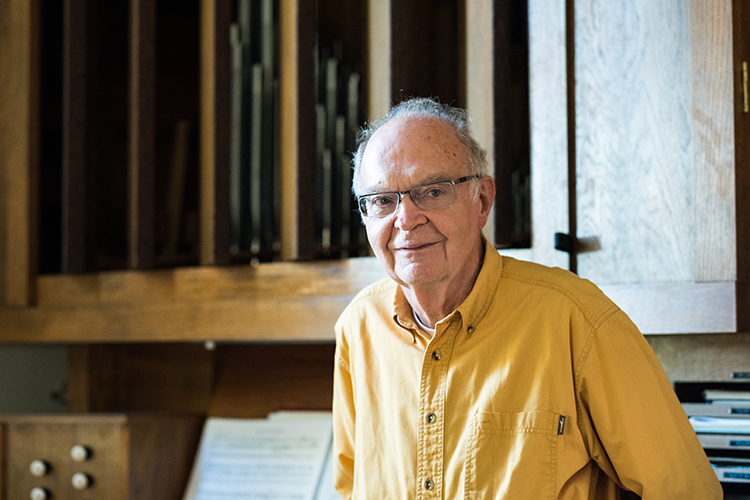
\includegraphics[scale=0.8]{Knuth-vivian20181019E.jpg}\\
        (2018 by Vivian Cromwell \cite{graphics})
    \end{center}
    }
    \only<2>{
    主な業績
    \begin{itemize}
        \item アルゴリズムの解析(計算量などによるアルゴリズムの定量的な評価を用いる)を計算機科学の研究分野として確立した
        \item ``The Art of Computer Programming'' の著作
        \item \TeX の開発
    \end{itemize}
    }
\end{frame}

\begin{frame}
    \frametitle{The Art of Computer Programming (TAOCP) \cite{taocp}}
    \large
    \begin{itemize}
        \item 種々のアルゴリズムの歴史、背景、アルゴリズム解析からの視点による解説書
        \item 当初は第7巻まで計画、現在第4巻の分冊まで刊行
        \item 30代前半までに最初の3巻の初版を刊行
    \end{itemize}
\end{frame}

\begin{frame}
    \frametitle{\TeX が生まれたきっかけ \cite{tex-wikipedia}}
    \large
    \begin{itemize}
        \item<1-> 1970年代後半、KnuthはTAOCPの改訂版に着手
        \item<2-> 初版は活版印刷で、ベテランの植字工による組版が行われていた
        \item<3-> 改訂版では電子写植のシステムに移行
        \item<4-> しかし、電子写植による数式などの組版の醜さに憤慨
        \item<5-> Knuth「それなら自分で計算機科学を用いて何かできるはず!」と決心
        \item<6-> 1978年のサバティカルの間に\TeX の開発に着手
        \item<7-> 一応の完成を見たのは1980年代終盤
    \end{itemize}
\end{frame}

\begin{frame}
    \frametitle{\TeX の特徴}
    \large
    \begin{itemize}
        \item プログラミング言語のように書物を作るシステム
        \item 文字も独自にデザインするシステムを同時に開発 (METAFONT)
        \item 文字(フォント)もKnuthが自らデザインした (Computer Modern Fonts)
        \item 「文芸的プログラミング」(Literate Programming) を実践
        \begin{itemize}
            \item プログラムとドキュメントを同時に記述し、プログラムの保守性と可読性を向上しようというアイデア
            \item \TeX と METAFONT のプログラムをこの手法で作成し、プログラムの解説本も出版
        \end{itemize}
    \end{itemize}
\end{frame}

\begin{frame}
    \frametitle{\LaTeX}
    \large
    \setstretch{1.5}
    \begin{itemize}
        \item Leslie Lamport が開発
        \item \TeX を基盤にした組版システム
        \item \TeX のマクロパッケージ(プログラムの集まり)で構成
        \item \TeX よりも手軽に組版できることを目指す
    \end{itemize}
\end{frame}

\begin{frame}
    \frametitle{MathJax \cite{mathjax}}
    \large
    \setstretch{1.5}
    \begin{itemize}
        \item \LaTeX や MathML などによる数式の表示をwebブラウザ上で行うためのJavascriptライブラリ
        \item 米国数学会 (American Mathematical Society) らによって開発が行われている
    \end{itemize}
\end{frame}

\begin{frame}
    \frametitle{参考文献}
    \begin{thebibliography}{99}
        \bibitem{graphics} D. E. Knuth. Downloadable Graphics. \url{https://www-cs-faculty.stanford.edu/~knuth/graphics.html} (参照 2019-06-30).
        \bibitem{taocp} D. E. Knuth. The Art of Computer Programming (TAOCP). \url{https://www-cs-faculty.stanford.edu/~knuth/taocp.html} (参照 2019-06-30).
        \bibitem{mathjax} MathJax. \url{https://www.mathjax.org/} (参照 2019-06-30).
        \bibitem{tex-wikipedia} Wikipedia. TeX. \url{https://ja.wikipedia.org/wiki/TeX}
         (参照 2019-06-30).
    \end{thebibliography}    
\end{frame}

\end{document}